% !TEX encoding = UTF-8 Unicode
\documentclass[a4paper]{article}

\usepackage{color}
\usepackage{url}
\usepackage[T2A]{fontenc} % enable Cyrillic fonts
\usepackage[utf8]{inputenc} % make weird characters work
\usepackage{graphicx}
\graphicspath{ {images/} }

\usepackage[english,serbian]{babel}
%\usepackage[english,serbianc]{babel} %ukljuciti babel sa ovim opcijama, umesto gornjim, ukoliko se koristi cirilica

\usepackage[unicode]{hyperref}
\hypersetup{colorlinks,citecolor=green,filecolor=green,linkcolor=blue,urlcolor=blue}

\usepackage{listings}

\usepackage{amsmath}
\usepackage{amsfonts}

% https://tex.stackexchange.com/questions/5223/command-for-argmin-or-argmax
\DeclareMathOperator*{\argmax}{argmax}

%\newtheorem{primer}{Пример}[section] %ćirilični primer
\newtheorem{primer}{Primer}[section]

\definecolor{mygreen}{rgb}{0,0.6,0}
\definecolor{mygray}{rgb}{0.5,0.5,0.5}
\definecolor{mymauve}{rgb}{0.58,0,0.82}

\lstset{ 
  backgroundcolor=\color{white},   % choose the background color; you must add \usepackage{color} or \usepackage{xcolor}; should come as last argument
  basicstyle=\scriptsize\ttfamily,        % the size of the fonts that are used for the code
  breakatwhitespace=false,         % sets if automatic breaks should only happen at whitespace
  breaklines=true,                 % sets automatic line breaking
  captionpos=b,                    % sets the caption-position to bottom
  commentstyle=\color{mygreen},    % comment style
  deletekeywords={...},            % if you want to delete keywords from the given language
  escapeinside={\%*}{*)},          % if you want to add LaTeX within your code
  extendedchars=true,              % lets you use non-ASCII characters; for 8-bits encodings only, does not work with UTF-8
  firstnumber=1000,                % start line enumeration with line 1000
  frame=single,	                   % adds a frame around the code
  keepspaces=true,                 % keeps spaces in text, useful for keeping indentation of code (possibly needs columns=flexible)
  keywordstyle=\color{blue},       % keyword style
  language=Python,                 % the language of the code
  morekeywords={*,...},            % if you want to add more keywords to the set
  numbers=left,                    % where to put the line-numbers; possible values are (none, left, right)
  numbersep=5pt,                   % how far the line-numbers are from the code
  numberstyle=\tiny\color{mygray}, % the style that is used for the line-numbers
  rulecolor=\color{black},         % if not set, the frame-color may be changed on line-breaks within not-black text (e.g. comments (green here))
  showspaces=false,                % show spaces everywhere adding particular underscores; it overrides 'showstringspaces'
  showstringspaces=false,          % underline spaces within strings only
  showtabs=false,                  % show tabs within strings adding particular underscores
  stepnumber=2,                    % the step between two line-numbers. If it's 1, each line will be numbered
  stringstyle=\color{mymauve},     % string literal style
  tabsize=2,	                   % sets default tabsize to 2 spaces
  title=\lstname                   % show the filename of files included with \lstinputlisting; also try caption instead of title
}

\begin{document}

\title{Automatsko prepoznavanje govora\\ \small{Seminarski rad u okviru kursa\\Metodologija stručnog i naučnog rada\\Matematički fakultet}}

\author{Vladimir Vuksanović, Aleksa Kojadinović, Lazar Čeliković\\kontakt email prvog, drugog, trećeg autora}

%\date{9.~april 2015.}

\maketitle

\abstract{
U ovom tekstu je ukratko prikazana osnovna forma seminarskog rada. Obratite pažnju da je pored ove .pdf datoteke, u prilogu i odgovarajuća .tex datoteka, kao i .bib datoteka korišćena za generisanje literature. Na prvoj strani seminarskog rada su naslov, apstrakt i sadržaj, i to sve mora da stane na prvu stranu! Kako bi Vaš seminarski zadovoljio standarde i očekivanja, koristite uputstva i materijale sa predavanja na temu pisanja seminarskih radova. Ovo je samo šablon koji se odnosi na fizički izgled seminarskog rada (šablon koji \emph{morate} da koristite!) kao i par tehničkih pomoćnih uputstava. Pročitajte tekst pažljivo jer on sadrži i važne informacije vezane za zahteve obima i karakteristika seminarskog rada.}
% Tema ovog rada je da priblizi citaoca zadatku automatskog prepoznavanja govora, problemima koji se javljaju i najznacajnijim arhitekturama ovih sistema.

\bigskip
\textbf{Ključne reči:} prepoznavanje govora

\tableofcontents

\newpage

\section{Uvod}
\label{sec:uvod}

Govor je za ljude najintuitivniji i prirodniji nacin komunikacije. Zbog toga je od samog nastanka kompjutera, nastala i ideja da koristimo isti nacin komunikacije da interagujemo sa njima.
To bi znatno smanjilo potrebno predznanje za koriscenje kompjutera i ucnilio ga pristupacnijim vecem broju ljudi. Najveca prepreka ovim sistemima do skoro je bio kako sa velikom tacnosti prepoznati sta je korisnik rekao.
Taj postupak se naziva automatsko prepoznavanje govora.

\textbf{Automatsko prepoznavanje govora} (eng.~{\em Automatic Speech Recognition, ASR}) je proces pretvaranja zvučnog signala govora u sekvencu reči pomoću kompjutera.
Neke od najznacajnijih primena ovih sistema su: pametni licni asistenti (Google Assistant\footnote{https://assistant.google.com/}, Apple Siri\footnote{https://www.apple.com/siri/},\dots), transkripcija snimaka, pretrazivanje audio sadrzaja i pristupacnost.
% slika

Iako su istrazivanja na ovu temu pocela jos sredinom dvadesetog veka, popularnost je pocela da dobija tek u poslednjoj deceniji kada je uvodjenje dubokih neuronskih mreza drasticno povecalo performanse ovih sistema.
Ta razlika je bila dovoljna da ucini ove sisteme prakticno primenljivim umesto nezgodnim za upotrebu zbog velikog broja gresaka.
Jedan od najznacajnijih postignuca je ostvareno 2016. godine je kompanija Majkrosoft napravila sistem koji je ostvario iste rezultate kao ljudski eksperti na transkripciji Switchboard skupa podataka \cite{switchboard}.
% Human level switchboard
% https://blogs.microsoft.com/ai/historic-achievement-microsoft-researchers-reach-human-parity-conversational-speech-recognition/
% https://www.microsoft.com/en-us/research/blog/microsoft-researchers-achieve-new-conversational-speech-recognition-milestone/
Za glavne uzroke ovog naglog poboljsanja se smatraju \cite{hannun2021history}:
\begin{enumerate}
  \item Sakupljanje velike kolicine tanskribovanih skupova podataka
  \item Nagli porast u performansama grafickih procesorskih jedinica (GPU)
  \item Poboljsanje algoritama za ucenje i arhitektura modela
\end{enumerate}
% The History of Speech Recognition to the Year 2030
% 1) the curation of massive transcribed data sets,
% 2) the rapid rate of progress in graphics processing units
% 3) the improvement in the learning algorithms and model architectures.

U nastavku cemo prvo navesti neke izazove koje treba da resimo da bi smo napravili dobar sistem za prepoznavanje govora, zatim cemo opisati nacin rada dva najpopularnija modela: statisticki i end-to-end i na kraju cemo predstaviti nacin za njihovu evaluaciju.

\section{Izazovi}
% https://www.youtube.com/watch?v=q67z7PTGRi8
Prepoznavanje govora je veoma težak zadatak zato što je potrebno da radi podjednako dobro u veoma različitim uslovima.
Neki od najvećih izazova su:
\begin{itemize}
  \item \textbf{Mala količina podataka za trening} --- 
  Za ostvarivanje dobrih rezultata potrebno je sakupiti više stotina ili čak hiljada sati labeliranih zvučnih snimaka koji treba da sadrže više govornika razlicitog pola i starosti, koji govore različitim akcentima. 
  Dok u skorije vreme jeste nastao porast u količini dostupnih podataka, veliki problem još uvek predstavlja reprezentativnost različitih varijacija u govoru i nedostatak podataka za jezike sa manjim brojem govornika. 
  Zbog toga se istražuju alternativni načini za treniranje kao sto su samo-treniranje (eng.~{\em self-training}) \cite{baevski2020wav2vec}, iterativno treniranje \cite{park2020noisy} ili treniranje koristeći kompjuterski generisan glas \cite{hannun2014deep}. 
  U dodatku \ref{sec:skupovi} se može naći tabela sa pregledom nekih od najpopularnijih trening skupova na engleskom jeziku.
  
  \item \textbf{Stil govora} --- 
  Postoje različiti sistemi u zavisnosti od toga koji tip govora mogu da prepoznaju \cite{anusuya2010speech}. Tipovi govora poređani po težini propoznavanja su: 
  \begin{enumerate}
    \item Izolovane reči --- reči su razdvojene dugim periodima tišine
    \item Povezane reči --- reči su razdvojene kratkim pauzama
    \item Neprekidan govor --- uvežbani govor, čitanje ili diktiranje
    \item Spontani govor --- neuvežbani, prirodni govor 
  \end{enumerate}
  Prve implementacije prepoznavanja govora su radile na nivou izolovanih reči i koristile su se za prepoznavanje određenih komandi ili cifara.
  Danas se najviše truda ulaže u poboljšanje prepoznavanja neprekidnog i spontanog govora.

  \item \textbf{Karakteristike govornika} ---
  Svaki čovek ima različitu boju glasa i govori različitom brzinom. Čak i starost osobe i jačina govora bitno utiču na frekvenciju glasa.
  Poseban problem pravi postojanje različitih dijalekata i akcenata koji mogu da imaju potpuno različite načine za izgovaranje istih reči.
  Jedan način za rešavanje ovog problema je treniranje sistema na glasu govornika koji će ga koristiti.
  To su sistemi zavisni od korisnika (eng.~{\em speaker dependent}) i koriste se u slučajevima da samo jedna osoba treba da ih koristi.
  Sa druge strane postoje sistemi nezavisni od korisnika (eng.~{\em speaker independent}) koji treba da rade podjednako dobro za sve govornike.
  
  \item \textbf{Okruženje govornika} --- 
  Ovi sistemi će retko biti korišćeni u potpuno tihim prostorijama sa profesionalnom opremom za snimanje. Zbog toga treba da budu tolerantni na različite vrste pozadinske buke ili kvaliteta mikrofona. 
  Neke vrste šumova je moguće otkloniti analizom zvuka ili naprednijim metodama \cite{xu2015enhancement}, ali jedan od najvećih problema predstavlja postojanje drugih govornika u okolini.
  Te signale je često teško razlikovati od glasa primarnig govornika, i samim tim teško ukloniti.
  
  \item \textbf{Veličina rečnika} --- 
  Povećanje broja reči koje model može da prepozna takođe povećava njegovu složenost i otežava treniranje, ali se time dobija na tačnosti. 
  Zbog toga je potrebno naći dobar kompromis između veličine rečnika i složenosti modela. 
  U slučajevima kada je potrebno pouzdano prepoznati samo neki skup komandi koriste se mali rečnici i oni su često veoma pouzdani, ali za prepoznavanje opšteg govora današnji sistemi su trenirani na skupu od oko 50.000-100.000 reči.
\end{itemize}

\section{Statisticki model}
\label{sec:statistical}

Dugo vremena statisticki pristup je bio dominantan za sisteme za prepoznavanje govora.
Iako je u skorije vreme pao u senku modela zasnovanih na dubokim neuronskim mrezama opisanim u poglavlju \ref{sec:e2e} ovaj model je jos uvek u sirokoj upotrebi i veoma vredan izucavanja.

% Large Vocabulary Continuous Speech Recognition a Review
Cilj ovih sistema je da pronadju najverovatniju transkripciju za zadati ulaz.
Formalno, neka je $\hat{W}$ optimalan niz reci za transkripciju nekog zvucnog signala $X$. Cilj je optimizovati formulu \cite{kamath2019nlp}:
\begin{equation*}
  \hat{W} = \argmax_{W} P(W|X)
\end{equation*}
primenom Bajesove formule to mozemo da zapisemo kao:
\begin{equation*}
  \hat{W} = \argmax_{W} \frac{P(X|W) P(W)}{P(X)}
\end{equation*}
a kako je $P(X)$ konstantno za konkretan ulaz, mozemo da ga eliminisemo:
\begin{equation}
  \label{eq:stat1}
  \hat{W} = \argmax_{W} P(X|W) P(W)
\end{equation}
Ideja je da umesto modeliranja $P(W|X)$ sto je tesko, odvojeno modeliramo verovatnoce iz prethodne formule za koje imamo bolje tehnike.

Najprirodniji nacin za racunanje $P(X|W)$ bi bio da se podeli na reci i za svaku od njih racuna verovatnoca da je izgovorena.
U nekim slucajevima, kao na primer kada treba prepoznati samo neki mali skup komandi, tada se i koristi ovaj pristup.
Problem nastaje u sistemima sa velikim vokabularom zato sto postoji veliki broj varijacija u izgovoru reci, a trening skup sadrzi mozda par primera za svaku od njih sto nije dovoljno da se dobro nauci njeno prepoznavanje.
Dakle, umesto na reci potrebna je finija podela i za to potrebu cemo koristiti foneme.
\textbf{Foneme} su najmanje jezicke jedinice na osnovu kojih mogu da se razlikuju znacenja vecih jedinica.
One postoje samo kao apstraktna ideja a njihova fizicka realizacija se zove glas.

Ako je $S$ niz fonema, $P(X|W)$ iz formule \ref{eq:stat1} se razlaze i dobija se:
\begin{equation*}
  \hat{W} = \argmax_{W} \sum_{S} P(X,S|W) P(W)
\end{equation*}
sto se moze aproksimirati kao:
\begin{equation}
  \label{eq:stat2}
  \hat{W} \approx \argmax_{W,S} P(X|S) P(S|W) P(W)
\end{equation}
Veličine iz prethodne formule imaju svoja imena na osnovu komponente koja ih računa:
$P(X|S)$ se naziva \textbf{akusticki model} (eng.~{\em acoustic model}), 
$P(S|W)$ je \textbf{model izgovora} (eng.~{\em pronunciation model}),
a $P(W)$ se zove \textbf{jezički model} (eng.~{\em language model})\footnote{Neka literatura $P(X|W)$ naziva akustičkim modelom, a model izgovora tretira kao njegov deo. U ovom radu će biti podrazumevano da su oni odvojeni modeli.}.

% https://www.idiap.ch/software/bob/docs/bob/bob.kaldi/stable/_images/ASR.png
Na slici \ref{fig:statistical_model} je prikazana cela struktura statistickog modela od zvucnog signala do transkripcije:
\begin{figure}[h!]
  \begin{center}
    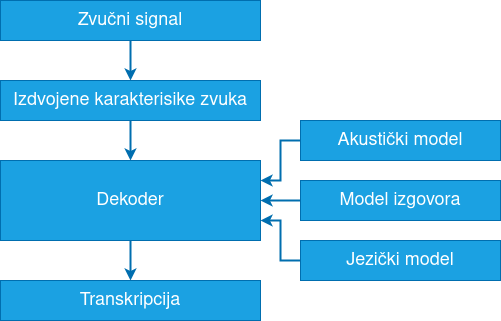
\includegraphics[scale=0.4]{statistical_model.png}
  \end{center}
  \caption{Statisticki model}
  \label{fig:statistical_model}
\end{figure}

U nastavku će biti opisana svaka od prikazanih komponenti, njena uloga i način rada.

\subsection{Obrada zvučnog signala}
Sirovi zvučni signal je veoma nepogodan za korišćenje zato što sadrži veliku količinu nebitnih informacija i šuma.
Zbog toga se, pre prosleđivanja akustičkom modelu, signal prvo obrađuje tako da ostanu samo ključne karakteristike i smanje šum i veličina reprezentacije.

Signal se deli na kratke segmente koji se zovu \textbf{okviri} (eng.~{\em frame}).
Svaki od njih je fiksne duzine (obično 10-30 milisekundi) sa kratkim preklapanjem sa susednim okvirima radi smanjenja naglih promena prilikom prelaska iz jednog u drugi.
Pretpostavka je da je u svakom okviru glas konstantan, to jest da se glasovi mogu menjati samo prelaskom iz jednog okvira u drugi.
Na svaki od tih novodobijenih delova se zatim primenjuje neka vrsta spektralne analize najčešće zasnovana na Furijeovoj transformaciji kojom se izdvajaju samo njegove najbitnije karakteristike.
Tačna reprezentacija koja se koristi varira u zavisnosti od modela, ali jedna od najpopularnijih je \textbf{MFCC} (Mel-Frequency Cepstral Coefficients) \cite{dave2013feature} zasnovana na Mel skali koja oponaša ljudski slušni sistem.
Ovako obrađen signal se prosleđuje akustičkom modelu.

\subsection{Akustički model}
% https://cs229.stanford.edu/section/cs229-hmm.pdf
% https://www.cs.cmu.edu/~roni/10601-slides/hmm-for-asr-whw.pdf
Akustički model je zadužen da pretvori obrađeni zvučni signal u niz fonema. 
Ovaj zadatak predstavlja idealan slučaj za primenu skrivenih Markovljevih modela \cite{rabiner1989hmm}.

\textbf{Skriveni Markovljev model} (eng.~{\em hidden Markov model}) je dinamički sistem kojeg karakteriše sledeće:
\begin{enumerate}
  \item $N$ skrivenih stanja $S = \{S_1, S_2, \dots, S_N\}$ pri cemu $q_t$ označava stanje u trenutku $t$
  \item $M$ obzervacionih simbola $V = \{V_1, V_2, \dots, V_M\}$ pri cemu $o_t$ označava obzervaciju u trenutku $t$
  \item Raspodela verovatnoća promene stanja predstavljena matricom $A=\{a_{ij}\}$ dimenzije $N \times N$ gde važi: $$a_{ij} = P(q_{t+1} = S_j | q_{t} = S_i) \quad 1 \leq i,j \leq N$$
  \item Raspodela verovatnoća obzervacionih simbola iz stanja $j$ predstavljena matricom $B=\{b_j(k)\}$ dimenzije $N \times M$ gde važi: $$b_j(k) = P(o_t = V_k | q_t = S_j) \quad 1 \leq j \leq N, 1 \leq k \leq M$$
  \item Raspodela inicijalnog stanja $\pi=\{\pi_i\}$ gde važi: $$\pi_i = P(q_1 = S_i) \quad 1 \leq i \leq N$$
\end{enumerate}
Primer jednog modela je prikazan na slici \ref{fig:hmm}.

\begin{figure}[h!]
  \begin{center}
    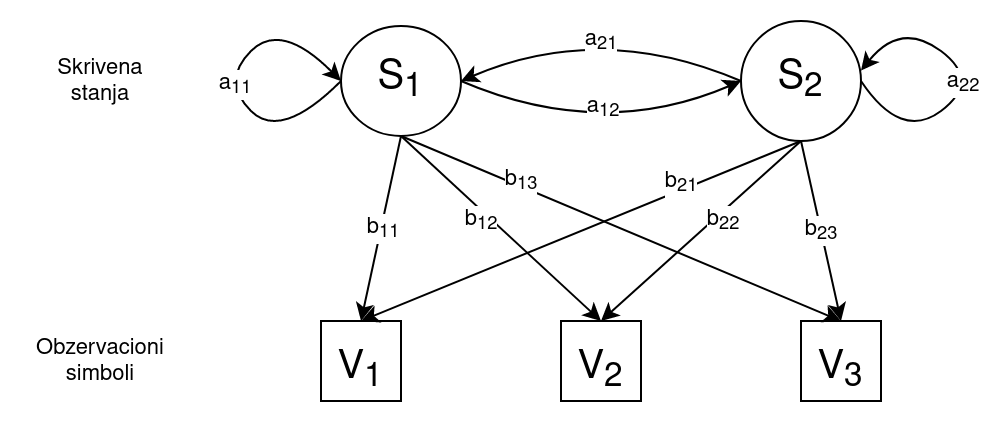
\includegraphics[scale=0.4]{hmm.png}
  \end{center}
  \caption{Primer skrivenog Markovljevog modela sa 2 stanja i 3 obzervaciona simbola}
  \label{fig:hmm}
\end{figure}

Konkretno za prepoznavanje govora, skriveni Markovljevi modeli se koriste za opisivanje svake foneme.
Svaki od njih se sastoji od nekog zadatog broja stanja (obicno 3 ili 5), a obzervacije su okviri zvučnog signala cije su verovatnoće predstavljene kao mešavina Gausovih raspodela.
Raspodele verovatnoća su dobijene treniranjem modela na skupu podataka.
Za svaku rečenicu iz trening skupa se konstruiše model spajanjem modela fonema u reči, pa reči u rečenicu.
Na njega se onda primeni Baum-Welch algoritam koji popravlja verovatnoće da više odgovaraju datim podacima.

Istrenirani model posle moze da predvidi najverovatniji niz fonema (stanja) za datu obzevaciju koristeci Vetrebi algoritam za pretragu.

\subsection{Model izgovora}
U prethodnoj sekciji je rečeno da se prilikom treniranja modeli fonema spajaju u modele reči, ali nije objašnjeno tačno kako se to radi.
To je baš zadatak modela izgovora.
On je u suštini veliki rečnik koji za svaku reč čuva niz fonema kako se ona izgovara.
Ako postoji više varijacija izgovora, one se smatraju kao ražlicite stavke u rečniku.
Sada konstrukcija modela reči postaje trivijalna, samo se pronađe njen izgovor u rečniku i nadovežu odgovarajuci modeli fonema.
Ukoliko se reč ne nalazi u rečniku, sistem za prepoznavanje govora neće biti u stanju da je prepozna.

Prirodno sledeće pitanje je kako se određuju ova preslikavanja. 
Ovo je zapravo jedan od najtežih zadataka za modeliranje zato što se on ne uči na skupu podataka nego ga konstruišu eksperti iz tog domena.
Za svaku reč, neko je morao da zapiše na koji način se izgovara uzimajući u obzir da potencijalno postoji više izgovora.
Sa obzirom da današnji sistemi razlikuju oko 100.000 reči, ovo nimalo nije lak posao.

\subsection{Jezički model}
Povratkom na formulu \ref{eq:stat2}, jezički model dodeljuje verovatnoću pojavljivanja $P(W)$ svakoj mogućoj sekvenci reči $W$.
Ovde se uzima u obzir relativna učestalost reči, verovatnoća da se reči nađu jedna za drugom, i mogu da se vrše dodatne sintaksne i semantičke provere.
Postoje rečenice koje zvuče slično ali nemaju sve semantičko znacenje.
Tada se od njih bira ona koja ima najviše smisla.
% primer

Kako $P(W)$ ne zavisi od zvucnog signala, moze se odvojeno trenirati na samo tekstualnom skupu podataka kojih postoji dosta vise i imaju veci broj primera od skupova sa transkribovanim snimcima.
U nekim slucajevima trenirana raspodela se moze promeniti u zavisnosti od korisnika (npr. pametni asistenti prepoznaju kontakte na korisnikovom telefonu).

Najvesci vid implementacije ovog modela je pomocu n-grama.
Neka se $W$ razdvaja na reci $W = \{w_1, w_2, \dots, w_m\}$ i neka je $n$ duzina n-grama.
To znaci da pri racunanju verovatnoce pojavljivanja neke reci u obzir uzimamo samo $n-1$ njenih prethodnika a za ostale pretpostavljamo da ne uticu.
Tada se $P(W)$ moze predstaviti kao:
\begin{equation*}
  P(W) = \prod_{i=1}^{m} P(w_i | w_1,\dots,w_{i-1}) = \prod_{i=1}^{m} P(w_i | w_{i-n+1},\dots,w_{i-1})
\end{equation*}
ako sa $C(x)$ oznacimo broj pojavljivanja sekvence $x$ u trening skupu tada se verovatnoca odredjene reci moze proceniti kao udeo pojavljivanja neke sekvence u broju pojavljivanja njenog prefiksa:
\begin{equation*}
  P(w_i | w_{i-n+1},\dots,w_{i-1}) = \frac{C(w_{i-n+1},\dots,w_i)}{C(w_{i-n+1},\dots,w_{i-1})}
\end{equation*}
Radi jednostavne implementacije na pocetak $W$ se dodaje $n-1$ "prazna" rec.

Sledeci problem je kako odrediti broj $n$.
On ne sme da bude preveliki zato sto se time smanjuje sansa da se neka kombinacija reci te duzine uopste nasla u trening skupu.
Cak i za male vrednosti moguce je da se neka sekvenca nije ranije videla. 
Taj problem se resava smanjenjem $n$ ukoliko ne postoji ta sekvenca duzine $n$ pa koriscenjem te verovatoce ili nekim postupkov ugladjivanja.

\subsection{Dekodiranje}
Konstrukcijom svih prethodno opisanih komponenti i njihovim treniranjem, model je gotov i spreman za upotrebu.
Jedino sto ostaje je pretraziti prostor dopustivih recenica da se pronadje ona koja najvise odgovara glasovnom signalu.
U praksi, taj prostor je veoma veliki i njegova pretraga je eksponencijalne slozenosti (svaka moguca kombinacija reci u recenici) stoga nije izvodljivo traziti egzaktno resenje.
Umesto toga se koristi heuristicki beam search algoritam. Ideja je da se resenje gradi iterativno i u svakom trenutku umesto testiranja svih mogucih puteva biramo $b$ najverovatnijih puteva.
Parametar $b$ se bira tako da balansira velicinu prostora za pretrazivanje i vreme potrebno za njegov obilazak.
Algoritam je dakle sledeci: odredimo verovatnocu za svaku rec da bude prva pa od njih izaberemo $b$ najverovatnijih. U sledecem koraku svaki od tih $b$ reci produzujemo sledecom i od njih ponovo biramo $k$ najverovatnijih.
Ovaj postupak se ponavlja sve dok ne dodjemo do kraja recenice i ona predstavlja konacnu transkripciju govora.

\section{End-to-end model}
\label{sec:e2e}
% prednosti u odnosu na HMM
% nije potreban ekspert za jezik
% lakse treniranje
% mogu sami da zakljuce bolju reprezentaciju od MFCC (npr pomocu CNN)

% mane u ondosu na HMM
% vice broj podataka

% modeli zasnovani na paznji i CTC modeli
\subsection{CTC model}

Neka je ulazni zvuk uzorkovan u proizvoljnom broju jednakih vremenskih intervala,  gde je svaki od njih predstavljen vektorom realnih brojeva duzine $m$.  Neka je $L$ konacna azbuka labela (oznaka).  Cilj je napraviti preslikavanje $h$ koje slika proizvoljan zvucni signal u niz labela:

\begin{equation}
\label{eq:pres1}
h: (\mathbb{R}^m)^* \rightarrow L^* 
\end{equation}


U praksi fiksiramo broj vremenskih trenutaka na neku vrednost $T$.  Iako je broj trenutaka fiksiran za zvucne signale,  nizovi labela ne moraju biti iste duzine za svaku ulaznu instancu, stoga jednu trening instancu predstavlja par $(\textbf{x}, \textbf{z})$ gde je $z$ vektor labela duzine najvise $T$.  Ako bismo test skup oznacili sa O, tada funkciju greske mozemo definisati na sledeci nacin:


\begin{equation}
\label{eq:LER}
LER(h, O) = \frac{1}{|O|}\sum_{(\textbf{x}, \textbf{z}) \in O}\frac{ED(h(\textbf{x}), \textbf{z})}{\textbf{|z|}}
\end{equation}


$ED$ predstavlja edit distancu (minimalni broj izmena koji dovodi jedan niz karaktera do drugog, pri cemu dozvoljene izmene podrazumevaju brisanje,  supstituciju i umetanje karaktera).  Prethodna mera naziva se stopa greske labela (\textit{eng.  label error rate - LER}).  


Formula \ref{eq:LER} jeste prirodna ocena greske za probleme koji za cilj imaju minimizaciju greske prevodjenja.

\bigskip
Koristeci sva prethodna razmatranja konstruisemo rekurentnu neuronsku mrezu koja na ulazu ima $mT$ ulaza,  dok se na izlazu dobija $T$ vektora dimenzija $L' = L \cup \{\epsilon\}$ pri cemu svaki predstavlja raspodelu verovatnoca oznaka za svaki trenutak prosirujuci azbuku blanko labelom $\epsilon$.

\bigskip
Neformalno receno,  prolaskom kroz izlazne softmax nizove dobijamo putanju $\pi \in (L')^T$ koja predstavlja jedan moguci odabir labela.  Ako $y_{\pi_t}^t$ predstavlja softmax ???? vrednost $t$-tog trenutka oznake $\pi_t$ tada verovatnocu odabira kompletne putanje dobijamo kao proizvod:

$$p(\pi|x) = \prod_{t=1}^Ty_{\pi_t}^t$$

U praksi uzorkovanje zvuka se vrsi u veoma sitnim vremenskim intervalima (oko 10ms). Stoga je pojava blanko ili dupliciranih oznaka veoma cesta.  Iz tog razloga uvodimo preslikavanje $\beta$ cija je uloga preciscavanje nizova labela uklanjanjem blanko oznaka i susednih duplikata.  

$$\beta : (L')^T \rightarrow L^U,  U \leq T$$

Primetimo da za jednu preciscenu putanju $l$ moze postojati vise mogucih izvornih putanja,  pa je verovatnoca njenog odabira jednaka sumi po svim izvornim putanjama.

\begin{equation}
\label{eq:beta}
p(l | x) = \sum_{\pi \in \beta^{-1}(l)} p(\pi | x)
\end{equation}

Imajuci u vidu sve prethodno navedeno,  zadatak preslikavanja $h$ je odabir najverovatnije preciscene putanje za dati ulaz.

\begin{equation}
\label{eq:h_x}
h(x) = \argmax_{l \in L^U} p(l | x)
\end{equation}

Najjednostavniji algoritam jeste pohlepni odabir najbolje oznake za svaki vremenski trenutak ponaosob.  Medjutim, ovakav pristup ne garantuje optimalnost.  Naravno,  postoje bolji algoritmi za resavanje datog problema. Isti nece biti obradjivani u ovom radu, ali se mogu naci u [].

\subsection{Modeli zasnovani na paznji}

Ovu grupu modela analiziramo na osnovu LAS (eng.  Listen Attend and Spell) modela.  Glavna razlika izmedju CTC modela i LAS modela ogleda se u odbacivanju pretpostavke o nezavisnosti u okviru niza oznaka.  

\bigskip
Glavne komponente ovog modola jesu Listener i Speller.  Okvirno gledano uloga listener komponente jeste da transformise ulazni signal u predefinisane karakteristike viseg nivoa (labele).  Takav izlaz prosledjuje se Speller komponenti koja konacno daje niz karaktera. 

\bigskip
Ubaci sliku

\bigskip

Slicno kao u poglavlju [] sa $\textbf{x}$ = $(x_1,  x_2,  ...,  x_T)$ oznacavamo ulazni signal.  $\textbf{y}$ predstavlja niz mogucih karaktera ukljucujuci razmak,  tacku,  zarez,  apostrof,  i tri specijalna karaktera (start - pocetak recenice,  stop - kraj recenice,  nep - nepoznat zvuk???).

\bigskip

Listener jeste rekurentna neuronska mreza piramidalne strukture.  Kao sto se moze primetiti na slici iznad broj neurona se u pravcu izlaznog sloja polovi.  Ova osobina nam omogucava smanjenje slozenosti izracunavanja,  sto je veoma pozeljno u slucaju kada je interval uzorkovanja veoma uzak.

\begin{figure}[h!]
  \begin{center}
    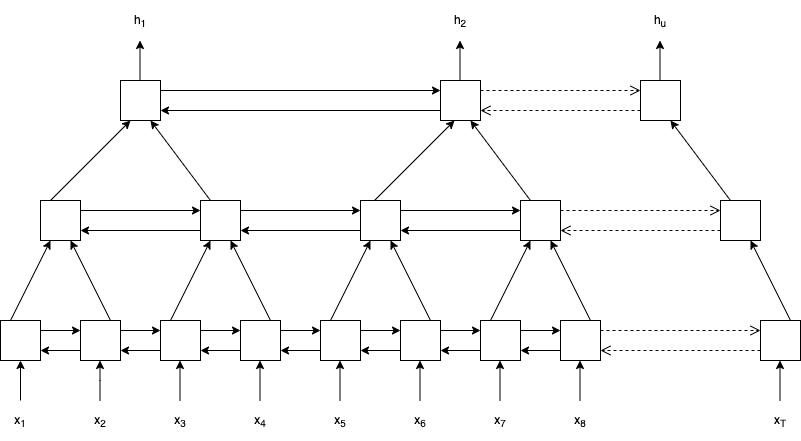
\includegraphics[scale=0.3]{listener.png}
  \end{center}
  \caption{Listener model}
  \label{fig:listener_model}
\end{figure}

\bigskip
Cilj je modelovati $\textbf{y}$ kao uslovnu raspodelu u zavisnosti od ulaznog signala $\textbf{x}$ i prethodnih izlaza $y_j,  j \in (1,  i-1)$

\begin{equation}
\label{eq:chain}
P(y | x) = \prod_i P(y_i | x,  y_j,  j < i)
\end{equation}

\bigskip

Speller je takodje rekurentna neuronska mreza.  Kao sto je vec pomenuto verovatnoca odabira svakog karaktera zavisi od odabira svih prethodnih.  Na izlaz $y_i$ utice stanje $s_i$ i kontekst $s_i$.  Stanje se racuna rekurentno na osnovu prethodnog stanja,  izlaza i konteksta.

 \begin{equation}
\label{eq:state}
s_i = RNN (s_{i-1},  y_{i-1},  c_{i-1})
\end{equation}

\begin{figure}[h!]
  \begin{center}
    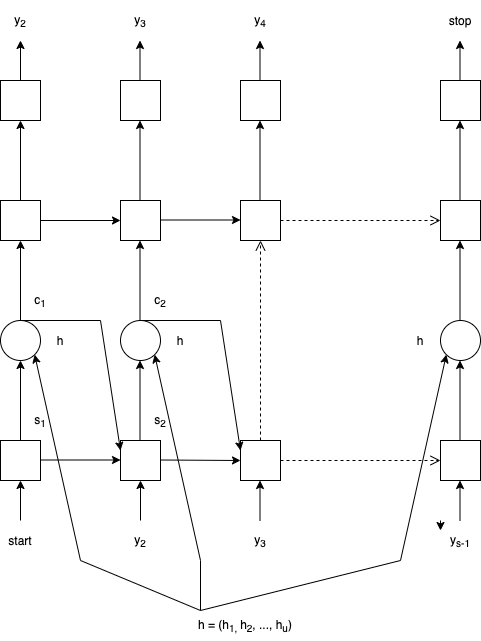
\includegraphics[scale=0.3]{speller.png}
  \end{center}
  \caption{Speller model}
  \label{fig:speller_model}
\end{figure}

\bigskip

Kontekst se izracunava koriscenjem standardnog mehanizma paznje (\textit{eng. Attention mechanism}).  Intuitivno, kontekst prikuplja relevantno znanje o okolnom ulaznom signalu potrebno za predikciju narednog karaktera,  na taj nacin odredjivajuci koliko znanje o okolini utice na znanje o trenutnom karakteru.

Treniranje se sprovodi odredjivanjem parametara koji maksimizaciju sumu uslovnih log verovatnoca za svaki karakter.

 \begin{equation}
\label{eq:max}
\max_{\theta} \sum_i \log P(y_i | x,  \bar{y}_j,  j < i; \theta)
\end{equation}

gde je $\bar{y_j}$ objektivna vrednost karaktera $j$.

Finalno dekodiranje vrsi se algoritmom beam pretrage (\textit{eng.  beam search}).  U koraku prosirivanja trenutnog cvora pretrage bira se $\beta$ najverovatnijih karaktera po verovatnoci dobijenoj na izlazu Speller komponente,  gde je $\beta$ parametar beam search algoritma.

\section{Metrike za evaluaciju}
Standardna mera za procenu kvaliteta sistema za prepoznavanje govora je \textbf{stopa pogrešnih reci} (eng.~{\em word error rate, WER}).
Za njeno izračunavanje potrebno je da imamo generisan tekst koji evaluiramo i tačnu transkripciju kao referencu.
Formula je izvedena normalizacijom Levenštajnovog rastojanja i izgelda ovako:
\begin{equation*}
  WER = \frac{I + D + S}{N}
\end{equation*}
gde je:
\begin{itemize}
  \item $I$ broj umetnutih reči
  \item $D$ broj obrisanih reči
  \item $S$ broj zamenjenih reči
  \item $N$ ukupan broj reči u referenci
\end{itemize}
Minimalna vrednost koju može da ima je 0, dok maksimalna vrednost može da bude preko 1 (npr. izgovorena je jedna reč a prepoznate dve).
Stopa pogrešnih reči se efikasno računa dinamičkim programiranjem, pomoću Vagner-Fišerovog algoritma (eng.~{\em Wagner-Fischer algorithm}). % čiji pseudokod se može naći u dodatku

Cilj sistema za prepoznavanje govora je da minimizuje ovu vrednost.

\section{Zaključak}
\label{sec:zakljucak}

% \section{Osnovna uputstva}
% Vaš seminarski rad mora da sadrži najmanje jednu \textbf{sliku}, najmanje jednu \textbf{tabelu} i najmanje \textbf{sedam referenci} u spisku literature. Najmanje jedna slika treba da bude originalna i da predstavlja neke podatke koje ste Vi osmislili da treba da prezentujete u svom radu. Isto važi i za najmanje jednu tabelu. 	Od referenci, neophodno je imati bar jednu \textbf{knjigu}, bar jedan \textbf{naučni članak} iz odgovarajućeg časopisa i bar jednu adekvatnu \textbf{veb adresu}. 
% \textbf{Dužina seminarskog rada treba da bude od 10 do 12 strana.} Svako prekoračenje ili potkoračenje biće kažnjeno sa odgovarajućim brojem poena. Eventualno, nakon strane 12, može se javiti samo tekst poglavlja \textbf{Dodatak} koji sadrži nekakav dodatni k\^{o}d, ali je svakako potrebno da rad može da se pročita i razume i bez čitanja tog dodatka. 

\addcontentsline{toc}{section}{Literatura}
\appendix
\bibliography{seminarski} 
% \bibliographystyle{plain}
\bibliographystyle{ieeetr}

\appendix

% dodatak: pregled skupa podataka za trening
% https://github.com/double22a/speech_dataset
% CommonVoice - https://commonvoice.mozilla.org/en/datasets
% TIMIT - https://catalog.ldc.upenn.edu/LDC93S1
% LibriSpeech - https://openslr.org/12/
% WSJ
% Fisher
\section{Dodatak: Pregled skupova podataka}
\label{sec:skupovi}

\begin{table}[h!]
\begin{center}
  % \caption{}
  \begin{tabular}{|c|c|c|c|c|}
    \hline
    Naziv skupa   & Duzina (sati) & Broj recenica & Broj govornika & Nivo transkripcije \\
    \hline
    TIMIT         & 5,4           & ?             & ?              & foneme, reci       \\ 
    Switchboard-1 & 260           & ?             & ?              & reci               \\ 
    LibriSpeech   & 100           & ?             & ?              & ?                  \\ 
    CommonVoice   & 2015          & ?             & ?              & ?                  \\
    GigaSpeech    & 10.000        & ?             & nepoznato      & reci               \\
    VoxPopuli     & 543           & 1313          & 413.581        & reci               \\
    \hline
  \end{tabular}
  % \label{tab:tabela1}
\end{center}
\end{table}

\end{document}

